%%%%%%%%%%%%%%%%%%%%%%%%%%%%%%%%%%%%%
%                                   %
% Compile with XeLaTeX and biber    %
%                                   %
% Questions or comments:            %
%                                   %
% joshua dot mcneill at uga dot edu %
%                                   %
%%%%%%%%%%%%%%%%%%%%%%%%%%%%%%%%%%%%%

\documentclass{beamer}
  % Read in standard preamble (cosmetic stuff)
  %%%%%%%%%%%%%%%%%%%%%%%%%%%%%%%%%%%%%%%%%%%%%%%%%%%%%%%%%%%%%%%%
% This is a standard preamble used in for all slide documents. %
% It basically contains cosmetic settings.                     %
%                                                              %
% Joshua McNeill                                               %
% joshua dot mcneill at uga dot edu                            %
%%%%%%%%%%%%%%%%%%%%%%%%%%%%%%%%%%%%%%%%%%%%%%%%%%%%%%%%%%%%%%%%

% Beamer settings
% \usetheme{Berkeley}
\usetheme{CambridgeUS}
% \usecolortheme{dove}
% \usecolortheme{rose}
\usecolortheme{seagull}
\usefonttheme{professionalfonts}
\usefonttheme{serif}
\setbeamertemplate{bibliography item}{}

% Packages and settings
\usepackage{fontspec}
  \setmainfont{Charis SIL}
\usepackage{hyperref}
  \hypersetup{colorlinks=true,
              allcolors=blue}
\usepackage{graphicx}
  \graphicspath{{../../figures/}}
\usepackage[normalem]{ulem}
\usepackage{enumerate}

% Document information
\author{M. McNeill}
\title[FREN2001]{Français 2001}
\institute{\url{joshua.mcneill@uga.edu}}
\date{}

%% Custom commands
% Lexical items
\newcommand{\lexi}[1]{\textit{#1}}
% Gloss
\newcommand{\gloss}[1]{`#1'}
\newcommand{\tinygloss}[1]{{\tiny`#1'}}
% Orthographic representations
\newcommand{\orth}[1]{$\langle$#1$\rangle$}
% Utterances (pragmatics)
\newcommand{\uttr}[1]{`#1'}
% Sentences (pragmatics)
\newcommand{\sent}[1]{\textit{#1}}
% Base dir for definitions
\newcommand{\defs}{../definitions}


  % Packages and settings

  % Document information
  \subtitle[Meubles et objets indirects]{Les meubles et les pronoms compléments d'objet indirect}

\begin{document}
  % Read in the standard intro slides (title page and table of contents)
  \begin{frame}
    \titlepage
    \tiny{Office: % Basically a variable for office hours location
Gilbert 121\\
          Office hours: % Basically a variable for office hours
 lundi, mercredi, vendredi 10:10--11:10
}
  \end{frame}

  \begin{frame}{À qui?}
    % dire, écrire, expliquer, parler, répondre, téléphoner
    % apporter, emprunter, prêter, remettre, rendre
    \begin{columns}
      \column{0.5\textwidth}
        \scriptsize
        On fait les choses suivantes à qui ou pour qui?
        \begin{enumerate}
          \item Loki leur donne un fauteuil du séjour.
          \item<2->[$\to$] Les Avengers
          \item<3-> Thanos lui montre ses jolies plantes dans le jardin.
          \item<4->[$\to$] Thor
          \item<5-> Spider-Man lui a offert un repas du four.
          \item<6->[$\to$] Hulk
          \item<7-> Dr Strange veut leur demander une étagère.
          \item<8->[$\to$] Les Avengers
          \item<9-> Jarvis et ses amis lui achètent un tapis pour son studio.
          \item<10->[$\to$] Black Widow
          \item<11-> Star-Lord leur a écrit la lettre sur la table basse de la chambre.
          \item<12->[$\to$] Les Avengers
        \end{enumerate}
      \column{0.5\textwidth}
        \begin{minipage}[t][0.6\textheight]{\linewidth}
          \begin{center}
            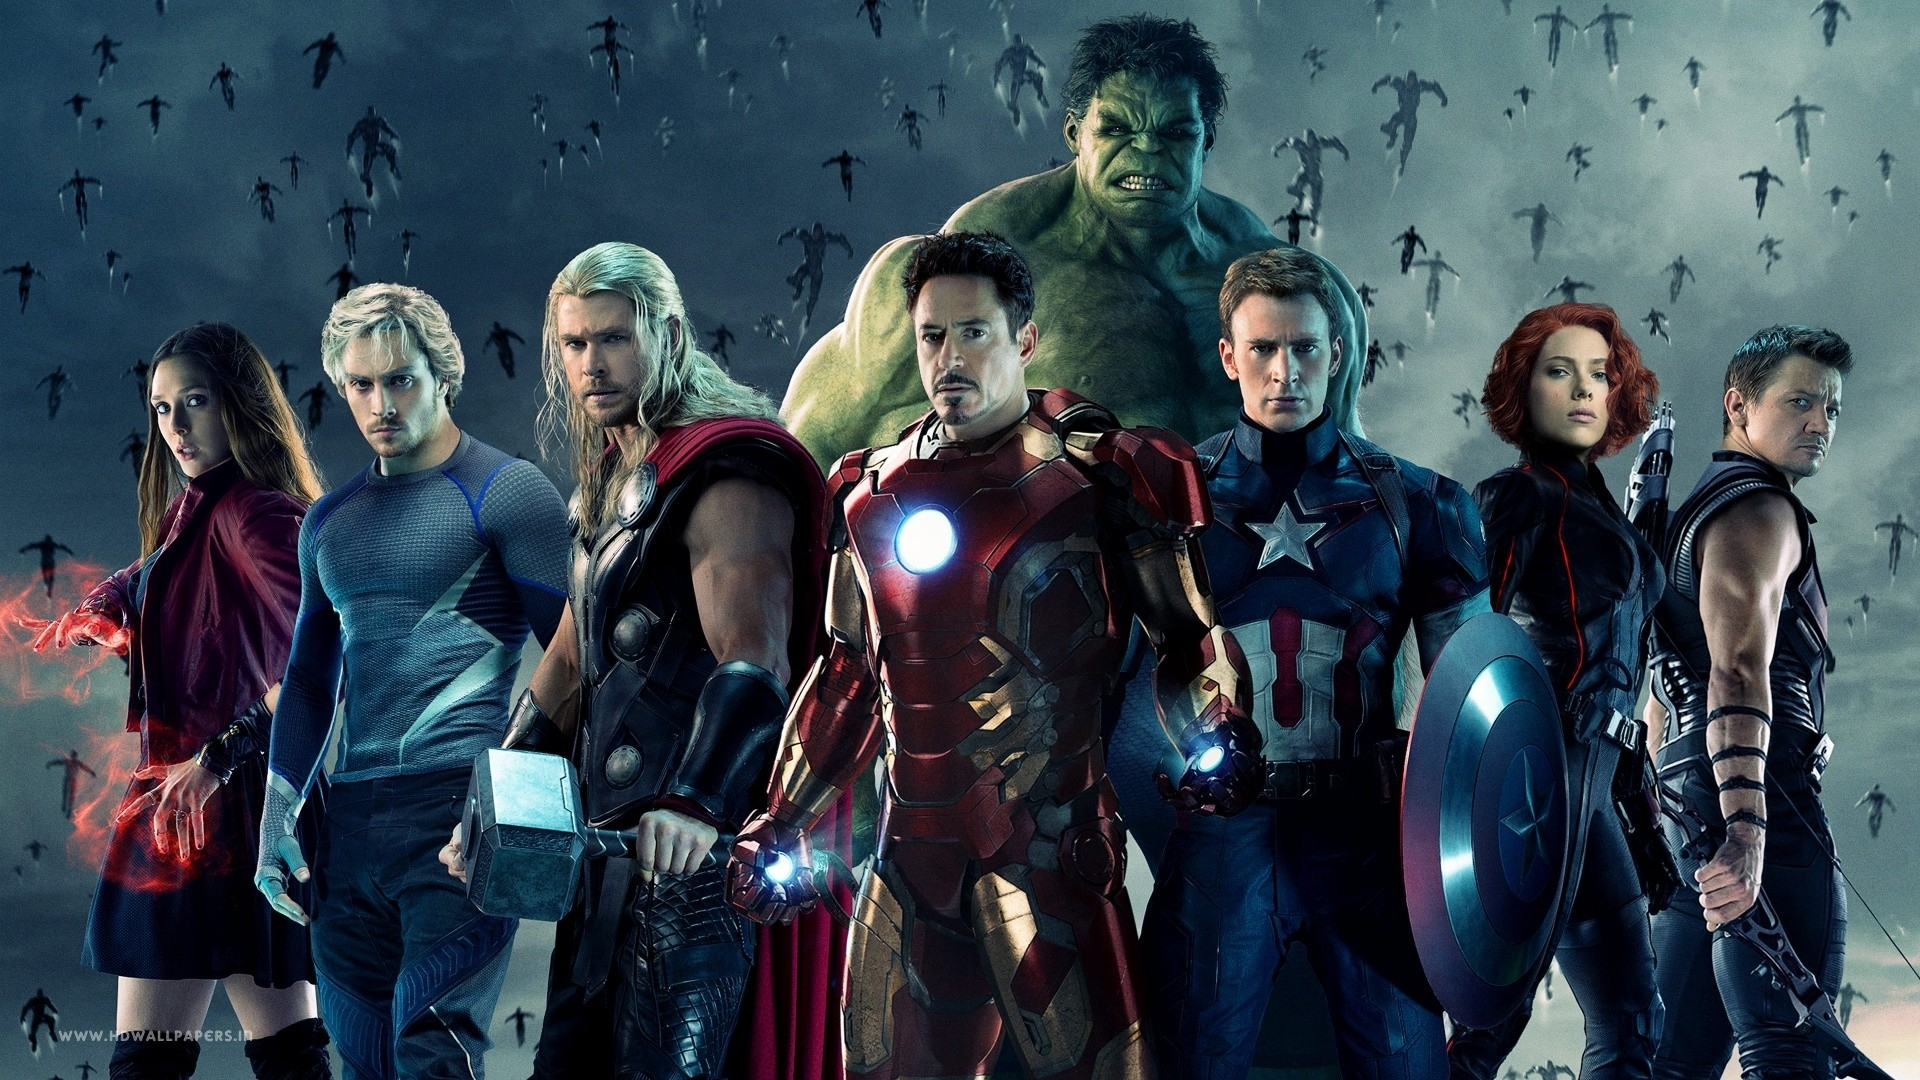
\includegraphics[scale=0.075]{avengers.jpg} \\
            ou \\
            \vspace{8pt}
            \only<1-2>{
              
\includegraphics[scale=0.1]{captain_america.jpg}
            }
            \only<3-4>{
              
\includegraphics[scale=0.03]{thor.jpg}
            }
            \only<5-6>{
              
\includegraphics[scale=0.1]{hulk.jpeg}
            }
            \only<7-8>{
              
\includegraphics[scale=0.09]{scarlet_witch.jpg}
            }
            \only<9-10>{
              
\includegraphics[scale=0.11]{black_widow.jpg}
            }
            \only<11-12>{
              
\includegraphics[scale=0.065]{iron_man.jpg}
            }
          \end{center}
        \end{minipage}
    \end{columns}
  \end{frame}

  \begin{frame}{}
    \begin{center}
      \Large Quiz
    \end{center}
  \end{frame}

  \begin{frame}{Rarement, souvent ou jamais?}
    Avec un/e partenaire, demande-lui avec quelle fréquence il/elle fait les choses suivantes.
    Utilise des adverbes comme \lexi{rarement}, \lexi{souvent}, \lexi{jamais} ou bien d'autres.
    \begin{description}
      \item[\textbf{Modèle:}] \emph{prêter tes vêtements à ta/ton colocataire}
      \item[E1:] Est-ce que tu prêtes tes vêtements à ta/ton colocataire?
      \item[E2:] Oui, je lui prête souvent mes vêtements!
    \end{description}
    \begin{columns}[t]
      \column{0.5\textwidth}
        \begin{enumerate}
          \item rendre les devoirs au professeur
          \item expliquer tes problèmes à ta mère
          \item téléphoner à tes parents
          \item offrir des cadeaux à ton père
        \end{enumerate}
      \column{0.5\textwidth} 
        \begin{enumerate}
          \setcounter{enumi}{4}
          \item demander de l'argent à tes parents
          \item emprunter des vêtements à ton/ta meilleur/e ami
          \item acheter des bonbons pour tes nièces et tes neveux
          \item emprunter de l'argent à tes amis
        \end{enumerate}
    \end{columns}
  \end{frame}

  \begin{frame}{Qu'est-ce qu'on peut offrir?}
    Les personnes suivantes ont acheté un nouvel appartement.
    Avec un/e partenaire, discutez ce que vous pourriez offrir comme cadeau.
    \begin{description}
      \item[\textbf{Modèle:}] \emph{Ma sœur n'a pas grand-chose aux murs.}
      \item[E1:] On peut lui offrir une belle affiche.
      \item[E2:] Oui, ou on peut lui offrir une photo de famille.
    \end{description}
    \begin{columns}[t]
      \column{0.5\textwidth}
        \begin{enumerate}
          \item Mes parents aiment bien les films.
          \item Mon oncle adore faire la cuisine.
          \item Ma tante adore travailler dans le jardin.
          \item Ma cousine aime lire.
        \end{enumerate}
      \column{0.5\textwidth} 
        \begin{enumerate}
          \setcounter{enumi}{4}
          \item Mes grands-parents aiment la musique.
          \item Mon cousin n'a pas de colocataire.
          \item Mes amis ont une belle terrasse.
        \end{enumerate}
    \end{columns}
  \end{frame}

  \begin{frame}{}
    \begin{center}
      \Large Questions?
    \end{center}
  \end{frame}
\end{document}
